\documentclass[a4paper,12pt,ngerman]{scrartcl}

% standard packages
\usepackage[german]{babel}
\usepackage[utf8x]{inputenc}
\usepackage[a4paper,margin=2.5cm]{geometry}

% additional packages
\usepackage[colorlinks=true,linkcolor=black,urlcolor=blue,
            citecolor=blue,anchorcolor=blue]{hyperref}
\usepackage{amsmath}
\usepackage{csquotes}
\usepackage{graphicx}
\usepackage{float}
\graphicspath{{bilder/}}

% specific packages which are less often needed
\usepackage[official]{eurosym}
\usepackage{tikz}
\usetikzlibrary{shapes,arrows}

% meta information
\title{Dosuas - Die Symphonie des Sehens}
\subtitle{Jugend Forscht 2018}
\author{Jonas Wanke und Yorick Zeschke}
\date{\today}

\begin{document}

\maketitle


\begin{abstract}
	Dosuas (\textbf{D}evice for \textbf{O}rientation in \textbf{S}pace \textbf{U}sing 
	\textbf{A}udio \textbf{S}ignals) ist ein Gerät, welches blinden Menschen ermöglicht
	sich mithilfe von Tonsignalen im Raum zu orientieren und Objekte zu erkennen.\par
	Das Projekt besteht aus zwei Unterprojekten, die beide bis zum 
	Wettbewerb als Prototypen umgesetzt werden sollen. Einmal werden Bilder eines 3D Kamera
	mit einem Programm in Töne umgewandelt, die dann mit 3D-Audio Kopfhörern hörbar gemacht
	werden. Die andere Idee basiert darauf, so ähnlich wie eine Fledermaus Ultraschall 
	Impulse zu senden und deren Reflektionen bzw. Echos hörbar zu machen, sodass man
	sich mit Klicklauten orientieren kann. Letzteres basiert auf der Technik der aktiven
	menschlichen Echoortung.
\end{abstract}

\tableofcontents

\newpage

\section{Einleitung}

Blinde Menschen haben schon immer Probleme damit, sich im Raum zu orientieren.
Manche von ihnen, zum Beispiel \textit{Daniel Kish} benutzen die Technik der 
\textit{menschlichen Echoortung}, ein Verfahren, bei dem
man regelmäßig mit dem Mund Klicklaute erzeugt und das Gehör darauf trainiert 
anhand der Reflektionen ein genaues Bild der Umgebung im Kopf zu erzeugen.
Forscher haben herausgefunden, dass sich dabei die Struktur des Gehirns verändert 
und Signale von den Ohren im Sehzentrum verarbeitet werden.
Mit genügend Übung schaffen es Blinde so zu \enquote{sehen} und können Fahrrad 
fahren oder in den Bergen klettern. \par 
Doch nicht jedem Blinden fällt es leicht und nicht jeder hat die Möglichkeit eine
solche Technologie zu erlernen. Außerdem hat auch die menschliche Echoortung ihre
Grenzen und ist ab einem bestimmten Punkt nicht mehr erweiterbar. Hier kommt die 
Technologie ins Spiel. Von Tag zu Tag ergeben sich neue Möglichkeiten mithilfe 
der verschiedensten technischen Hilfsmittel Menschen das Leben zu erleichtern.
Geräte wie 3D-Sensoren oder Kameras können heutzutage schon oft sehr realistische
und detaillierte Bilder aufnehmen, die dem menschlichen Sehen sehr nahe kommen. \par 
Relativ neu ist zum Beispiel die Technologie der Retina Implantate, die sich 
momentan aber noch im Anfangsstadium der Entwicklung befinden. Mit ihnen soll es in 
Zukunft möglich sein, dass Blinde wie nicht sehbehinderte Menschen sehen, jedoch
können die Kosten von 75.000 \euro{} aufwärts selten von den Blinden selbst getragen
werden und werden nur manchmal von Krankenkassen übernommen. Auch gibt es zu viele
blinde und sehbehinderte Menschen, als dass es möglich wäre jeden mit einem so 
teuren Gerät zu versorgen.\par 
Andere Firmen versuchen das Sehen technisch durch andere Sinne zu ersetzen.
Ein berühmtes Beispiel dafür ist der 
\enquote{BrainPort V100}\footnote{https://www.wicab.com/brainport-v100}, welcher 
Kamerasignale in elektronische Impulse umwandelt, die auf der Zunge spürbar
gemacht werden. Nachteile dieser
Technologie sind vor allem lange Lernprozesse, die nur mit ärztlicher Unterstützung
möglich sind, Probleme bei zu vielen Reizen oder große Ungenauigkeiten.
Beispielsweise kann es passieren, dass ein Blinder beim Betrachten des Geschehens auf 
einer großen Straße nichts mehr wahrnimmt, weil der Tastsinn der Zunge
nicht für eine 
solche Reizüberlastung ausgelegt ist. Im Gegensatz dazu wird es vermutlich auch nicht
möglich sein kleine oder komplexere Objekte zu erkennen, weil der Tastsinn der Zunge
dazu wiederum nicht sensibel genug ist. \par
Weil unser Gehirn sehr anpassungsfähig ist und beeindruckende
Leistungen im Finden von Regelmäßigkeiten oder Mustern erbringt, ist der Ansatz
andere Sinne zu verwenden eine vielversprechende Strategie. Darauf setzt auch 
unser Projekt, Dosuas, welches den Hörsinn verwenden möchte um Blinden eine Hilfe
für Orientierung und Erkennung der Umwelt zu geben.

\newpage

\section{Echoortungsstrategie}

\subsection{Funktionsweise}

Die Echoortungsstrategie funktioniert ähnlich einem Sonar. Hierbei werden im einfachsten 
Fall Schallwellen in eine Richtung ausgesendet, von verschiedenen Oberflächen reflektiert,
und danach wieder empfangen. Über die Zeit, die die Schallwellen benötigen, kann die 
Entfernung zu einem Gegenstand nach der Formel $d = \frac{t \cdot c}{2}$ ermittelt werden,
wobei $d$ die Entfernung, $t$ die gemessene Zeit, und $c$ die Schallgeschwindigkeit (in 
diesem Fall im Medium Luft) sind. Die Halbierung kommt daher, dass der Schall die 
Entfernung zum Objekt doppelt zurücklegt (hin und zurück). \par
In unserem Fall wurde zur Messung zunächst ein einfacher Ultraschallsensor\footnote{HC-SR04} 
verwendet. Dieser wird über eine fallende Eingangsflanke getriggert, und gibt nach einer 
kurzen Zeit einen Puls mit der Länge der gemessenen Zeit aus. Die Triggerung übernimmt 
beim Prototypen der Einfachheit halber ein Microcontroller\footnote{Arduino Micro}, die 
Ausgabe erfolgt direkt über einfache Kopfhörer. Der Puls, der hier gehört werden kann, 
wird je nach Entfernung als ein (bei sehr kurzen Enfternungen, $0,03m < d < 0,2m$) oder 
zwei schnell aufeinanderfolgende (bei größeren Enfternungen, $0,2m < d < 4m$) klick-ähnliche 
Laute wahrgenommen. Diese Laute werden bei den beiden Flanken des Pulses erzeugt, die Dauer 
dazwischen verhält sich somit proportional zur gemessenen Entfernung. Mit etwas Übung kann 
diese Entfernung grob geschätzt werden, sodass Objekte mit ausreichender Größe vor einer 
Person erkannt werden. \par
Dieser Puls enthält aber nur noch Informationen über den dichtesten Gegenstand, dessen 
reflektiertes Signal einen Schwellwert überschreitet. Grund hierfür ist die Filterung im 
Ultraschallsensor. Im zweiten Schritt soll nun diese Filterung übergangen werden, indem 
das Ausgangssignal davor abgegriffen wird. Somit werden auch kleinere Pulse (also von 
kleineren Flächen) sowie insgesamt mehrere Pulse (bei mehreren Objekten) an die Kopfhörer 
ausgegeben. Außerdem hat der Ausgangspuls des Sensors normalerweise eine festgelegte 
Intensität, welche hier jedoch je nach Größe der Fläche variieren kann. Um sich hiermit 
orientieren zu können ist allerdings mehr Übung erforderlich. \textbf{TODO: Praxistest} \par
Der dritte Schritt ist nun ein Stereosound. Bisher wurde nur erkannt, ob sich in einer 
gewissen Entfernung ein Gegenstand befindet. Man weiß hierbei aber nicht, ob dieser direkt 
vor einem, eher auf der linken oder eher auf der rechten Seite ist. Um dieses Problem zu 
lösen wird ein zweiter Empfänger verwendet, wobei die Empfänger nun direkt über den Ohren 
platziert werden müssen (aber trotzdem nach vorne zeigen). Der Transmitter befindet sich 
mittig auf der Stirn. Somit wird ein ausgesendetes Signal von beiden Seiten empfangen, je 
nach Position der reflektierenden Fläche jedoch mit leicht abweichenden Intensitäten und 
Verzögerungen. Das menschliche Gehör funktioniert ähnlich, indem es durch diese 
Intensitätsdifferenzen und Laufzeitunterschiede die Richtung einer Audioquelle ermitteln 
kann\footnote{Es gibt noch eine dritte Methode, die vom Gehör verwendet wird. Hierbei wird 
durch feine Klangvariationen, die durch Reflexionen am Kopf und an den Ohren auftreten, die 
Richtung noch genauer bestimmt. Nur dadurch kann zwischen vorne-rechts und hinten-rechts 
sowie oben und unten unterschieden werden. Da die Messungen jedoch zunächst nur nach vorne 
gehen, wird diese Methode vernachlässigt.}. Somit sollte es auch mit dem Ultraschall noch 
relativ schnell möglich sein, seine Umgebung zu ''sehen''. \textbf{TODO: Praxistest}

\subsection{Fazit}

Das Verfahren ist der menschlichen Echoortung sehr ähnlich, jedoch muss der Mensch hierbei 
die Laute nicht selbst erzeugen. Da in diesem Fall Ultraschall verwendet wird, kann das 
Verfahren auch in lauten Umgebungen eingesetzt werden, und stört in ruhigen Situationen 
niemanden. Die Echoortung ist preisgünstig und einfach umzusetzen, kann aber je nach 
Umfang nur ungenaue Angaben treffen. Die komplexeren Varianten benötigen wiederum eine 
längere Übungszeit.

\newpage

\section{3D Kamera Strategie}

\subsection{Funktionsweise}

In diesem Teilprojekt werden die Daten einer 3D Kamera als Töne kodiert, die der Träger des Geräts
dann verwenden kann um ein Gefühl für den ihn umgebenden Raum zu bekommen. 

\subsubsection{Verwendete Technologien}

Der wichtigste Teil dieses Projekts ist eine ToF (Time of Flight) Kamera, die neben normalen Fotos 
auch sogenannte Tiefenbilder aufnehmen kann.
In einem Tiefenbild bekommt jeder Pixel einen Wert, der die Entfernung zur Kameralinse in mm angibt.
Der von uns verwendete \enquote{Cube Eye MDC500C}\footnote{http://www.cube-eye.co.kr/en/\#/spec/product\_MDC500d.html}
Sensor hat eine Reichweite von 0.8 bis 5.3 Metern und eine Auflösung von 320x240 Tiefenpixeln. 
Time of Flight Kameras messen die Entfernung mit Infrarotlicht. Deshalb funktioniert der Sensor auch 
im Dunkeln und wird von normalen Lichtreflektionen nicht gestört. Trotzdem hat der Sensor Probleme beim
Erkennen von lichtdurchlässigen oder reflektierenden Objekten (z.B. Glasscheiben oder Spiegel). Für einen
Prototypen ist das aber kein großes Problem. Wir haben diese Kamera ausgewählt, weil sie uns von einem 
Familienmitglied\footnote{Jan Nicklisch, Vater von Yorick Zeschke, arbeitet in der Firma
	\enquote{DILAX}, die diese Sensoren für Personenzählsysteme verwendet} 
empfohlen wurde.\par
Einen weiteren wichtigen Teil des Projekts stellen 3D-Audio Kopfhörer dar. Diese können den Eindruck
erzeugen, dass sich eine Tonquelle im dreidimensionalen
Raum befindet, bzw. sich bewegt. Dieses Verfahren benutzen wir um dem Träger des Geräts einen Eindruck
davon zu geben in welcher Richtung sich ein Objekt befindet.\par 
Die dritte Komponente ist ein \enquote{Raspberry Pi}, ein 
Einplatinencomputer, auf dem ein Linux-Betriebssystem läuft. Dieser ist mit Kopfhörern und dem ToF Sensor 
verbunden und führt unser Programm aus. Wir verwenden den Raspberry Pi, weil er klein, mobil und 
stromsparend ist.\par 
Zusammen ergeben die drei Bestandteile (und eine mobile Stromquelle) einen Prototypen, den wir zum Ausstellungstag vorführen werden.

\subsubsection{Softwarestruktur}

Das Programm ist in C++ geschrieben, weil die API des ToF Sensors C++ erfordert und C++ eine hardwarenahe
Sprache mit vielen Möglichkeiten ist. Wir verwenden folgende Libraries:
\begin{enumerate}
	\item \textit{MTF API} - eine Schnittstelle mit der man den Cube Eye Sensor ansteuern kann
	\item \textit{PCL} - eine Bibliothek um mit Punktwolken\footnote{Punktwolken sind (ggf. geordnete) Mengen von Punkten im dreidimensionalen Raum, 
		wobei jeder Punkt eine x-, y- und z-Koordinate und einen Index bekommt} zu arbeiten, wir benutzen 
	sie für Bildverarbeitung der 3D Daten
	\item \textit{SFML} - eine einfache Multimedia Bibliothek, 
	die wir für das Abspielen von 3D Sounds verwenden 
\end{enumerate} 
Die Software selbst besteht im Moment aus 3 Modulen, die sich aber bis zur Ausstellung noch verändern 
können.
\begin{enumerate}
	\item \textit{sensorReader.cpp} - ein Modul, das die Schnittstelle zum ToF Sensor benutzt um Daten zu 
	lesen und in eine Struktur für die weitere Verarbeitung zu bringen
	\item \textit{imageProcessor.cpp} - ein Modul zum Umwandeln der 3D Daten in eine Punktwolke und 
	Vorbereiten bzw. Verarbeiten der Punktwolke
	\item \textit{audioPlayer.cpp} - ein Modul, welches die Vorbereiteten Daten in Töne umrechnet und 
	diese dann abspielt
\end{enumerate}

Den Sourcecode finden Sie auf https://github.com/YpsilonZett/Dosuas.

\subsubsection{Programmablauf}

Die Software läuft kontinuierlich in einer Schleife, bis sie beendet wird und macht alle 6 Sekunden ein 
Tiefenbild. Dieses wird vom Sensor als 2D Matrix von 320$\,$x$\,$240 (=76.800) natürlichen Zahlen dargestellt.
In diesem Tiefenbild gibt jeder Pixel den Abstand zur nächsten lichtreflektierenden Region in mm an. 
Dadurch erscheint eine gerade Fläche direkt vor dem Sensor jedoch auf dem Bild als nach außen gekrümmt, 
weil das vom Sensor gesendete Infrarotlicht zu den Seiten der Fläche (und zurück) ein bisschen länger
braucht als zur Mitte. Wegen der kugelförmigen Ausbreitung der Lichtstrahlen von der Kameralinse hat das
Bild außerdem ein Polarkoordinatensystem\footnote{jeder Pixel gibt eigentlich einen Winkel zwischen
	0$^{\circ}$ und 75$^{\circ}$ an, weil der Sensor ein Sichtfeld von 75$^{\circ}$ hat}, mit dem wir nicht
gut weiterarbeiten können. Um das Problem der Verzerrung zu beheben und das Bild in ein kartesisches
Koordinatensystem umzurechnen verwenden wir einen Undistortion\footnote{in unserem Fall einen
	vom Hersteller mitgelieferten, den man direkt in der Sensorkonfiguration einstellen kann} Algorithmus. Danach wird das Bild in eine Punktwolke mit kartesischem Koordinatensystem umgerechnet.\par
\begin{figure}[H]
	\centering
	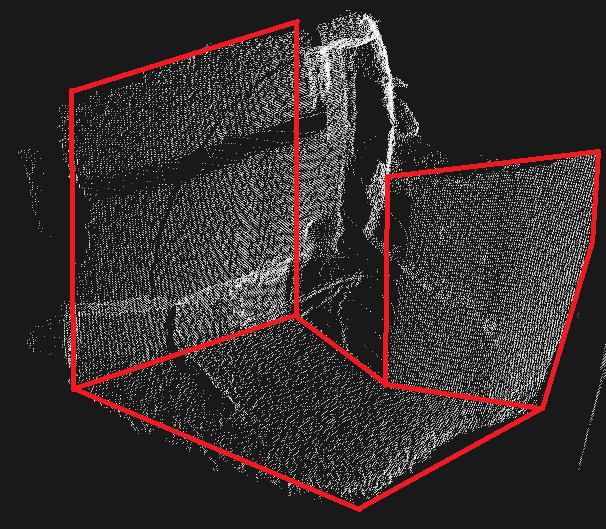
\includegraphics[width=0.6\textwidth]{no_undistortion2}
	\caption{verzerrte Punktwolke mit Messfehlern, vor dem Undistortion-Algorithmus}
	\label{distorted_pointcloud_img}
\end{figure}
Wie in Abb. \ref{distorted_pointcloud_img} zu sehen ist, wirkt ein ebene Fläche wie ein Teil der Oberfläche einer Kugel. Mit Rot sind hier ungefähr die Flächen im Bild
markiert, damit Sie ein Gefühl für die Orientierung bekommen. Dieser Raum enthält eine Menge 
Flächen und ist relativ einfach aufgebaut. Deshalb eignet er sich gut als Testumgebung.
\begin{figure}[H]
	\centering
	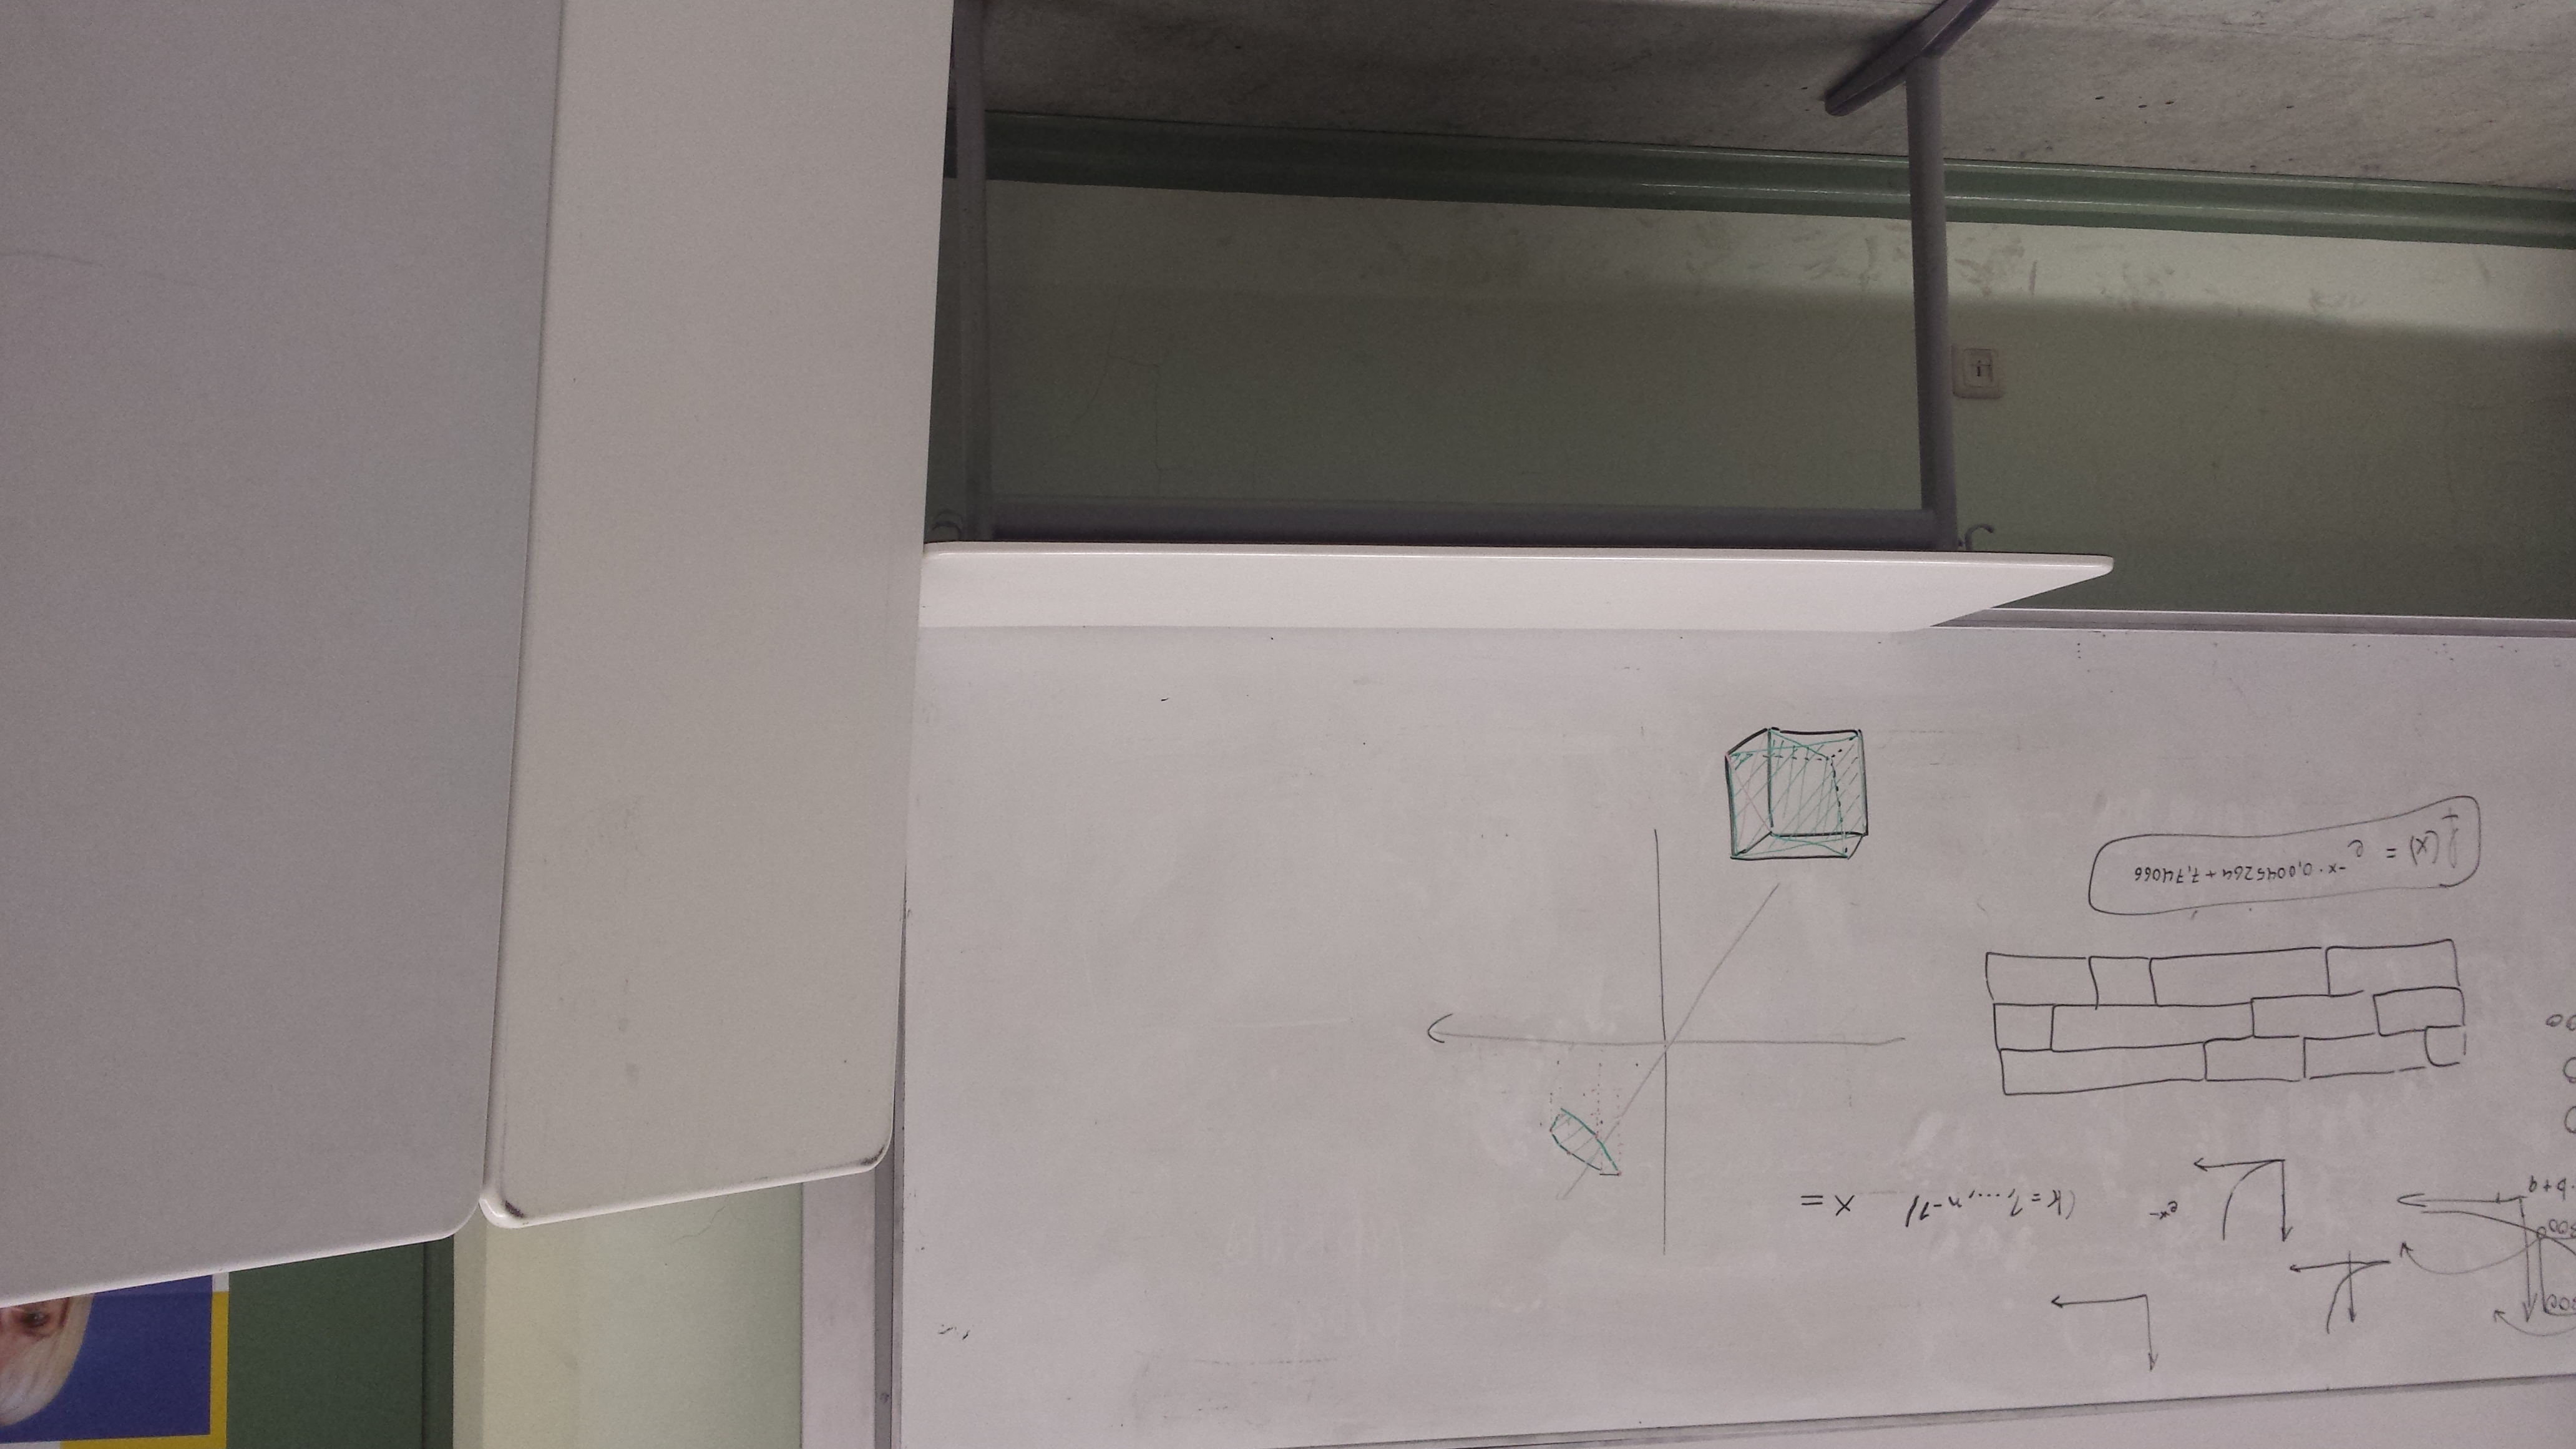
\includegraphics[angle=180,width=0.6\textwidth]{20180125_171703}
	\caption{Kamerabild des Raumes aus Abb. 1}
	\label{room_at_school}
\end{figure}
\par In der nächsten Abbildung (Abb. \ref{before_filtering}) sieht
man die Aufnahme des selben Zimmers, in der die Wände gerade erscheinen.
\begin{figure}[H]
	\centering
	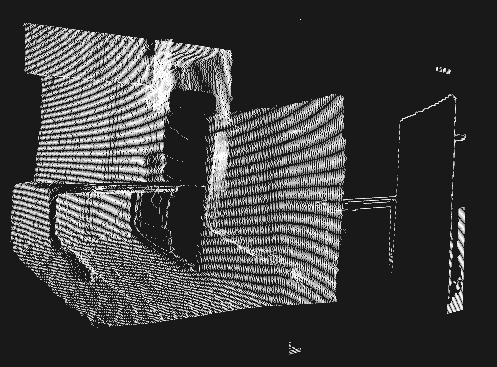
\includegraphics[width=0.6\textwidth]{before_filtering}
	\caption{algorithmisch korrigierte Punktwolke ohne Verzerrung}
	\label{before_filtering}
\end{figure} \par
Nachdem die Punktwolke korrigiert wurde, werden Boden und Decke entfernt, weil diese Fehler in 
der späteren Bildverarbeitung hervorrufen würden. Momentan filtern
wir einfach alle Voxel heraus, deren y-Koordinate kleiner als 40 oder größer als 200 ist\footnote{Koordinaten auf der y-Achse gehen von 0 (oberer Bildrand) bis 240 (unterer Bildrand)}. Diese naive Methode soll später durch das Entfernen von Boden und Decke mit dem Flächenfindungsalgorithmus RANSAC geschehen. Hier sehen Sie eine Punktwolke nach der
Filterung. Diese enthält nur noch ungefähr 62800 Punkte.
\begin{figure}[h]
	\centering
	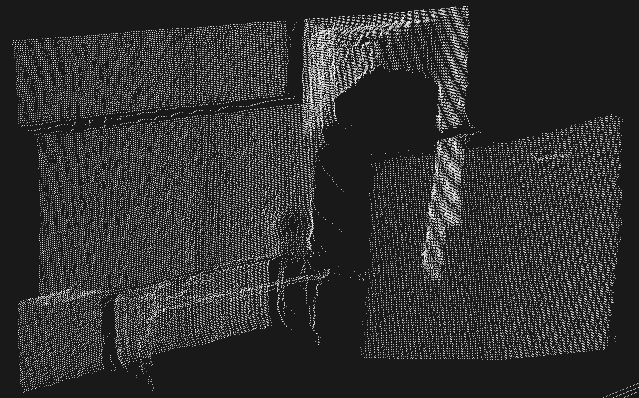
\includegraphics[width=0.6\textwidth]{after_filtering}
	\caption{Punktwolke nach Filtern und Entfernen von Decke bzw. Boden}
	\label{after_filtering}
\end{figure}
\par
Einmal wird die Punktwolke dann noch gefiltert, um ihre Größe zu reduzieren. 
Diese Art von Filterung nennt man Downsampling. Wir verwenden dafür den \enquote{VoxelGrid} Algorithmus der \enquote{\textbf{P}oint \textbf{C}loud \textbf{L}ibrary}.
Weil VoxelGrid die Punktwolke mithilfe eines Durchschnittsverfahrens reduziert, 
werden statistische Anomalien und Extremwerte ausgefiltert. Ein Bild mit genauer Auflösung eignet sich für unseren Zweck nicht so gut, wie ein niedriger
auflösendes, denn bei hoher Auflösung können kleine oder ungewöhnlich geformte Regionen (z.B. Messfehler, kleine Gegenstände, Kanten, Ecken, etc.) beim Hören
einen ungewollten Eindruck erzeugen. Das geschieht, weil unser Gehör sehr stark auf 
Änderungen in einem regelmäßigen Ton, wie wir ihn im Normalfall hören wollen, reagiert. 
Hier sehen Sie wieder den selben Raum, nur dass die Punktwolke diesmal nur noch aus ungefähr 15650 (also ca. ein Fünftel der ursprünglichen Größe) Punkten besteht. 
\begin{figure}[h]
	\centering
	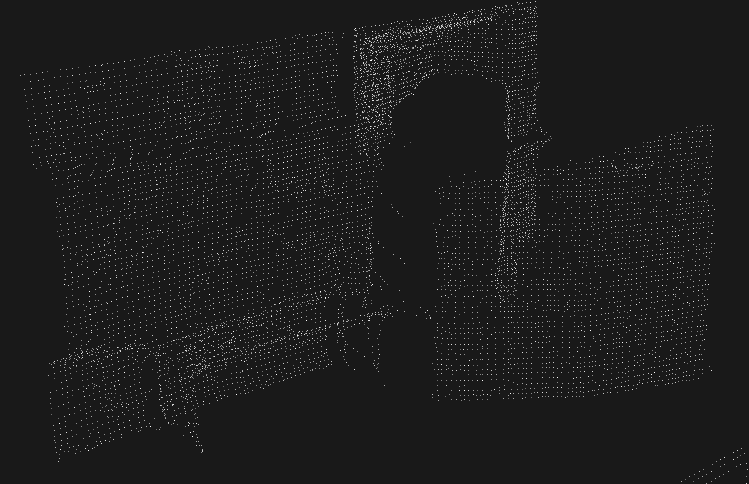
\includegraphics[width=0.6\textwidth]{after_downsampling}
	\caption{Punktwolke nach Downsampling mit geringerer Auflösung}
	\label{after_downsampling}
\end{figure}
\par 
Nach der Filterung wird das Bild in 320 vertikale Spalten unterteilt, die jeweils 240 Pixel hoch sind. 
Für jede Spalte wird aus den 5 \enquote{nächsten} (auf den den Träger bezogen) Voxels\footnote{so bezeichnet man einen dreidimensionalen Pixel mit x, y und z-Koordinaten} ein Voxel berechnet,
dessen z-Koordinate (Tiefe) der Durchschnitt der 5 anderen Voxel ist. Seine x-Koordinate entspricht
der Spaltennummer und die y-Koordinate ist ebensfalls der Durchschnitt der anderen 5 y-Koordinaten. 
320 dieser Voxel ergeben einen radarscannähnlichen Streifen (horizontal) mit Tiefen- und 
Höheninformationen. Dieser wird für das Tonabspielen benutzt.\par 
Ein Ton, wir nennen ihn \enquote{Radar Swipe}, weil er einem Radarscann durch das ganze Bild ähnelt, 
bewegt sich immer vom linken zum rechten Rand des Sicht-, bwz. Hörfeldes und ändert dabei (meistens) fortwährend
seine Frequenz. Durch diese wird eine Entfernung angegeben\footnote{tiefe Töne entsprechen großer 
	Entfernung und hohe Töne einem nahen Objekt}. Zusammen mit der Position\footnote{diese ist virtuell,
	hört sich aber wegen der Kopfhörer sehr realistisch an}, welche man über
die 3D-Audio Kopfhörer mitbekommt, kann man sich mit etwas Übung ein gutes Bild der Umgebung und ihrer
Beschaffenheit machen. Zum Beispiel könnte ein Ton, der in der linken Bildhälfte langsam tiefer wird und 
in der rechten Bildhälfte gleich bleibt eine schräge Wand darstellen, die in einiger Entfernung in eine
zum Nutzer parallele Wand übergeht. So ein einfaches Beispiel kommt zwar selten vor, und meistens gibt es
noch eine Menge Störgeräusche, aber näheres dazu im Abschnitt \ref{testsAndResults}.\par 
Momentan beträgt die Dauer zum Abspielen eines Bildes fünf Sekunden, gefolgt von einer Sekunde 
Pause. Bis zum Wettbewerb wollen wir die Dauer noch verkürzen, jedoch erfordert das ein gewisses 
Training, weil der Mensch üben muss, mehr Informationen in kürzerer Zeit zu verarbeiten. Zusammen mit 
einer Verkürzung der Pausen zwischen Aufnahmen hoffen wir die Zeit für einen Programmzyklus auf ungefähr
eineinhalb bis drei Sekunden zu reduzieren. 

\subsection{Praxistests} \label{testsAndResults}

Wir haben Dosuas in verschiedenen Umgebungen getestet und planen eine Vorführung am Ausstellungstag.
Es stellte sich heraus, dass sich zum Üben der Handhabung des Gerätes mittelgroße Räume mit einfachen
Formen besser eigenen. Die Räume dürfen aber nicht zu groß sein, weil der Sensor eine maximale Reichweite
von 5,3 Metern hat. Auch in zu kleinen Räumen eignet sich das Gerät nicht, denn der Sensor hat eine  Mindestreichweite von 0,8 Metern. Am Anfang sind Räume ohne viele kleine Objekte und mit großen 
Flächen wie Wänden einfacher, weil die Töne gleichmäßiger sind.
Hier sieht man einen anderen Raum, an dessen Beispiel wir die Töne beschreiben wollen, die man
mit unserem Gerät hören würde.
\begin{figure}[h]
	\centering
	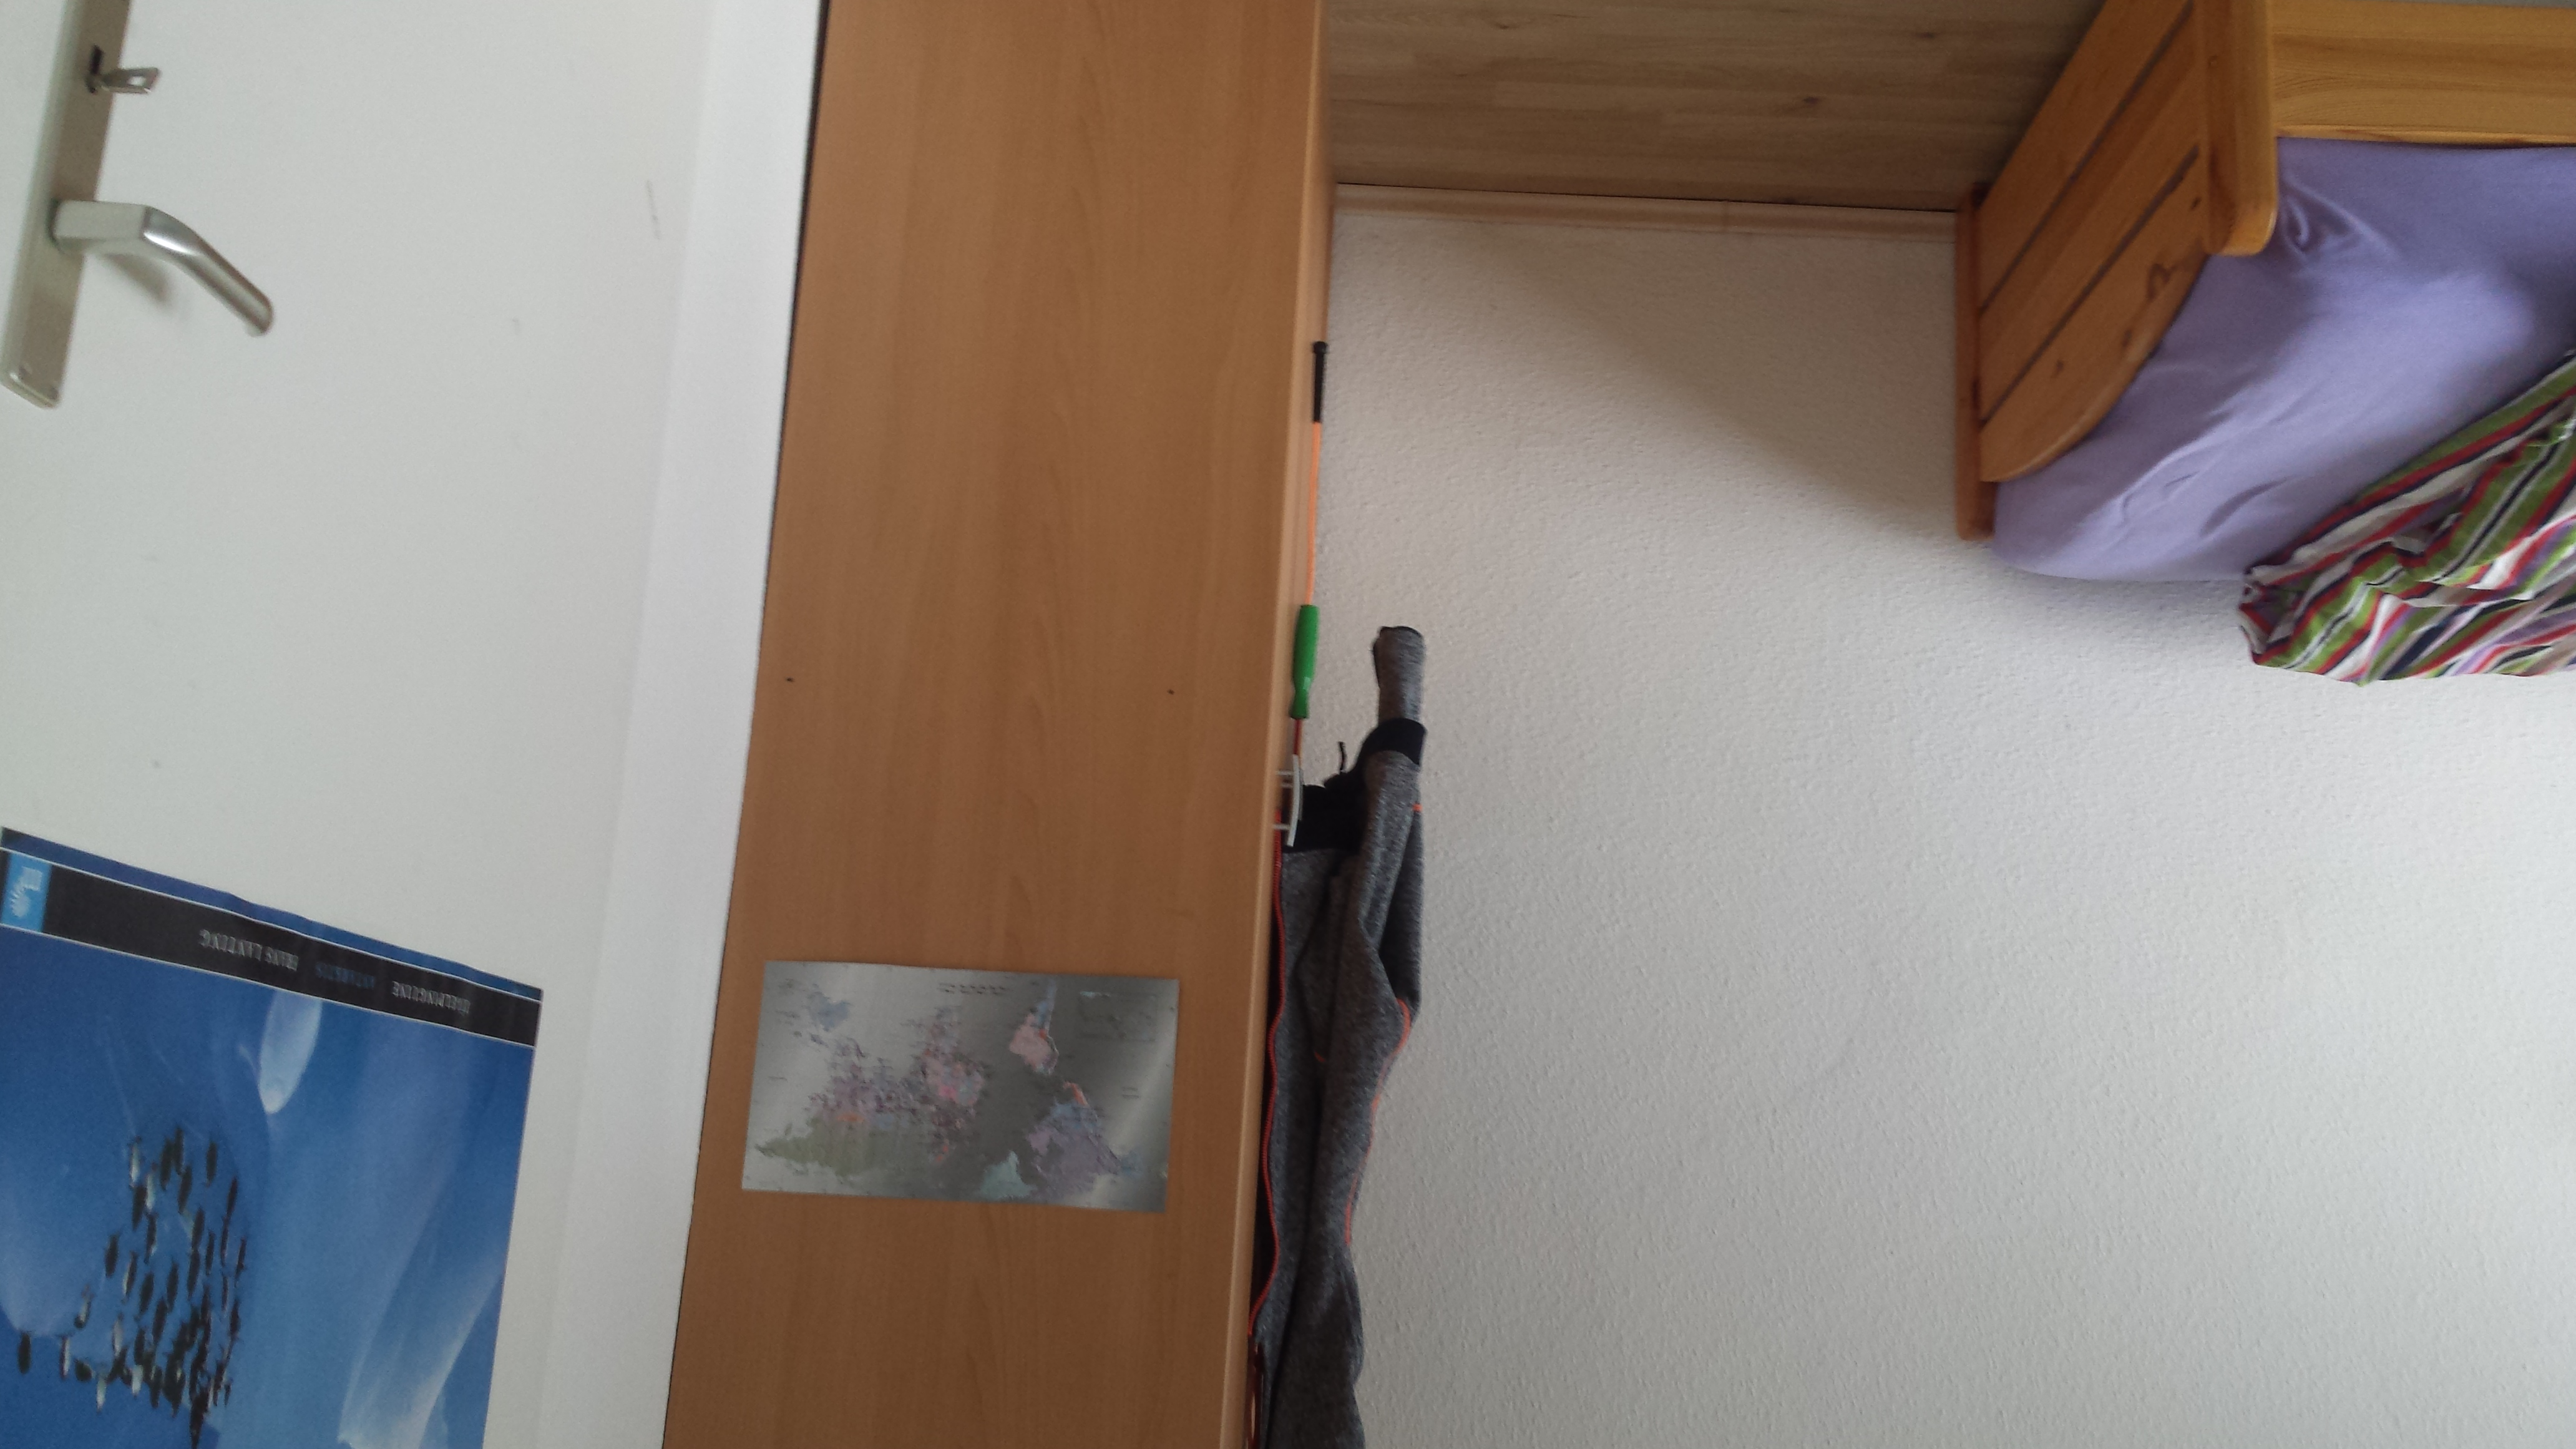
\includegraphics[angle=180,width=0.6\textwidth]{20180120_114953}
	\caption{Kamerabild eines anderen Raumes}
	\label{normal_picture}
\end{figure} \par
Man hört beim Betrachten dieses Raumes einen Ton, der ungefähr eine halbe Sekunde die Frequenz (von ca. 550Hz) nicht verändert und sich so anhört, als würde er von links kommen. Dieser Ton wird durch das Bett
erzeugt. Als nächstes wird der Ton über ungefähr eine halbe Sekunde gleichmäßig Tiefer (bis auf 340Hz), 
jetzt ist unsere virtuelle Tonquelle an der Wand des Raumes angekommen. Der Ton steigt nun über $1\frac{1}{2}$ Sekunden sehr langsam an (bis ca. 360Hz), denn die Wand hat eine leichte Neigung. 
erzeugt. Als nächstes wird der Ton über ungefähr eine eine halbe Sekunde gleichmäßig tiefer (bis auf 340Hz), 
jetzt ist unsere virtuelle Tonquelle an der Wand des Raumes angekommen, und steigt dann über $1\frac{1}{2}$ Sekunden sehr langsam an (bis ca. 360Hz), denn die Wand hat eine leichte Neigung. 
Nun hört man eine Art Sprung, bei dem der Ton ruckartig von 360Hz zurück auf 550Hz wechselt. An solchen Auffälligkeiten kann man Kanten, Öffnungen oder spitze Gegenstände erkennen, was sehr wichtig für Blinde
ist. Dieser Ton repräsentierte nämlich den Übergang von der Wand zum Schrank, der weiter vorne ist. Außerdem hört
man die virtuelle Tonquelle in diesem Moment direkt in der Mitte des Hörfeldes, was dem Nutzer anzeigt, das sich
die Kante fast genau vor ihm befindet. Über ungefähr eine Sekunde bleibt die Tonhöhe wieder gleich, nur die Position
verändert sich; man hört die Fläche des Schranks. Über die restlichen $1\frac{1}{2}$ Sekunden steigt der Ton mit 
gleichbleibender Geschwindigkeit an und die Tonquelle wandert nach rechts.
Hier hört man die Tür und am Ende eine kurze \enquote{Spitze}, die die Türklinke darstellt. Am Ende hat der Ton
eine Frequenz von ca. 790Hz.\par 
Wir hoffen, dass Sie sich nun ein Bild davon machen können, wie sich die Welt mit Dosuas anhört. Nach einem
halbstündigen Selbsttraining mit dem Gerät war unsere Testperson\footnote{Yorick Zeschke hat den ersten Prototypen
getestet} in der Lage (natürlich mit verbundenen Augen) in Schulräumen und Gängen
Wände und Türen zu erkennen, deren Ausrichtung und Entfernung er beschreiben konnte, ohne sie gesehen zu haben.
Außerdem war er in der Lage zu sagen ob eine Tür offen, halboffen oder geschlossen ist. Nach einer weiteren Stunde
war es ihm möglich Menschen, Tische und deren ungefähre Ausrichtung zu bestimmen. 
Wir haben bereits einige wiederkehrende Muster gefunden, die auf bestimmte Objekte in einem Raum hindeuten. 
\begin{figure}[h]
	\begin{tabular}{| p{0.4\textwidth} | p{0.5\textwidth} |}
		\hline
		Objekt & Beschreibung des Tons \\ \hline
		Wand oder große Fläche & verändert gleichmäßig und ununterbrochen seine Tonhöhe \\ \hline
		Kante, Ecke, sehr steile Fläche oder spitzer Gegenstand & \enquote{Sprung} von einer Tonhöhe zu einer 
		anderen \\ \hline
		Tür, Öffnung oder Loch & gleichmäßiger Ton (z.B. Wand), dann Sprung (Kante), wieder gleichmäßiger Ton
		(z.B. Gang hinter der Tür), noch ein Sprung und dann wieder ein gleichmäßiger Ton (Wand geht weiter) \\ \hline 
		Mensch oder Säule & gleichmäßiger Ton (z.B. Wand), dann \enquote{kreisförmiger}\footnotemark Ton, dann wieder gleichmäßiger Ton \\ \hline
		unregelmäßiges Objekt (z.B. Gardrobe mit Kleidung oder Computer auf einem Tisch) & zitternd\footnotemark erscheinender Ton \\ \hline 
	\end{tabular}
\end{figure} \par
\footnotetext{Intuitiv würde man so einen Ton wahrscheinlich
	als kreisförmig beschreiben. Die Frequenzänderung kann durch eine nach unter geöffnete gestreckte Parabel angenähert werden.}
\footnotetext{weil der Ton schnell zwischen verschiedenen Frequenzen wechselt} 
Wir wollen das Gerät noch mit
anderen Leuten testen und sehen, wie schnell jemand lernt, damit umzugehen. Wir vermuten, dass man nach einigen 
Tagen Selbsttraining im Stande ist, ohne Hilfe durch noch nie gesehene Räume zu gehen, ohne dabei irgendwo an zu
stoßen und den Weg nach draußen wieder zu finden. Längeres Üben oder technische Verbesserungen bieten ungeahnte
Möglichkeiten. Doch das Gerät ist und bleibt momentan nur ein Prototyp. 

\newpage

\section{Diskussion}

Im folgenden wollen wir kurz diskutieren, was wir für das Projekt planen und inwiefern man das
Gerät benutzten und weiterentwickeln kann und sollte. Außerdem fassen wir die durch die Entwicklung und Forschung am Projekt Dosuas gewonnenen Erkenntnisse im Fazit zusammen. 

\subsection{Ausblick}

Es gibt noch sehr viele Möglichkeiten das Projekt weiterzuentwickeln. Einige vielversprechende,
möchten wir hier auflisten. Die Entwicklungen sind nach ihrer Schwierigkeit und Entwicklungsaufwand geordnet. Einige sind auch nur Ideen.
\begin{enumerate}
	\item algorithmisches Entfernen von Decke, Boden und störenden Objekten
	\item Verbesserung der Genauigkeit des Tons, z.B durch größeres Frequenzspektrum, kein 
	VoxelGrid Filter mehr
	\item Einbauen von Höhenwahrnehmung durch besseres 3D Audio oder andere Effekte
	\item Erfassen des ganzen Bildes und nicht nur eines Streifens (die im Moment gehörten
	Voxel bilden einen Streifen, weil pro Spalte im Bild nur ein Voxel genommen wird), dies
	kann z.B. durch Tonüberlagerungen, Schwebungen, Akkorde Tonlautstärke oder unterschiedliche
	Klangfarben realisiert werden
	\item Benutzten eines auf das Projekt angepassten Sensors, der dadurch günstiger wird
	\item Benutzten mehrerer Sensoren für 3d Sichtfeld (wir können aus jeder Richtung Töne hören,
	warum nicht diese Fähigkeit verwenden?)
	\item Verkleinern und besser portabel machen des Geräts 
	\item und vieles mehr...
\end{enumerate}
Viele der hier aufgezählten Entwicklungen werden wir bis zum Wettbewerb wahrscheinlich nicht 
mehr schaffen. Aber dieser Ausblick dient auch als Ideen für Leute, die nach Jugend Forscht 
daran interessiert sind, das Projekt weiter zu entwickeln. Vermutlich werden wir das Projekt
dann als Open Source Projekt veröffentlichen.

\subsection{Fazit}

Im Moment fehlen uns noch genügend Messdaten um eine aussagekräftige Statistik zu machen. Jedoch
können wir mit Sicherheit sagen, das erste Schritte wie das Herumlaufen in fremden Räumen mit
dem jetzigen Stand möglich sein sollten. Wirklich \enquote{Sehen} können Leute mit dem Gerät
noch nicht und der Weg bis dahin ist noch weit, aber etwas ebenfalls sehr wichtiges
ist bereits möglich: Erkennen. Mit Dosuas kann man sich im Raum orientieren, Strukturen einfacher und später auch komplexerer Objekte erkennen und die Form von Gegenständen erahnen. Also tut das Gerät genau das, was sein Name sagt, es ist ein Gerät zur Orientierung im Raum mithilfe von Audio
Signalen, ein \enquote{\textbf{D}evice for \textbf{O}rientation in \textbf{S}pace \textbf{U}sing 
	\textbf{A}udio \textbf{S}ignals}.\par 
Das Gerät ist natürlich kein Ersatz für menschliches Sehen, aber das war am Anfang der Entwicklung
auch gar nicht beabsichtigt. Das Projekt Dosuas sollte eine Hilfestellung für Blinde sein, die ihnen das Leben einfacher macht. Kleine und genaue Gegenstände kann man mit unserem jetzigen Sensor nicht besonders gut erkennen. Das muss man aber auch nicht, denn dazu besitzen wir Menschen den Tastsinn, der wesentlich genauer ist. Auch sonst ist es nicht beabsichtigt, sich auf 
ein Gerät wie dieses zu verlassen. Man kann alltägliche Prozesse mit Dosuas einfacher machen. 
Wir hoffen das dieses oder ähnliche Projekte mehr blinde Menschen dazu motiviert, sich nicht 
mit ihrer Behinderung wie mit einer Last abzumühen, sondern Geräte oder Techniken
,wie z.B. menschliche Echoortung, zu verwenden um nicht mehr auf ständige Hilfe angewiesen 
zu sein und selbständiger zu werden. Wie Daniel Kish in einem TED-Talk\footnote{https://www.ted.com/talks/daniel\_kish\_how\_i\_use\_sonar\_to\_navigate\_the\_world} sagte, 
empfindet er Blindheit nicht als Problem, sondern als Eigenschaft, die ihn von anderen Menschen
unterscheidet. Diesem Beispiel sollten unserer Meinung nach mehr Blinde folgen.\par 
Vielleicht wird Dosuas irgendwann die Grundlage für ein weiteres
Forschungsprojekt sein, das es blinden Menschen vollständig ermöglicht zu sehen. Bis dahin
warten wir gespannt und versuchen mit unserem Projekt den Grundstein dafür zu legen. 

\newpage

\section{Anhang}

\end{document}